\chapter{Inleiding}
\label{inleiding}
Het reconstrueren van fresco's waarvan in opgravingen fragmenten gevonden worden is een moeilijke taak. Men kan het vergelijken met het oplossen van een enorme puzzel waarvan de stukken arbitraire vormen hebben, de meesten hun originele kleur zijn verloren en er vele anderen ontbreken. Daarbovenop ondervinden veel fragmenten erosie over de eeuwen heen, waardoor ze niet meer perfect op elkaar passen en confirmatie nog moeilijker wordt.\\

\begin{figure}[ht]
	\begin{center}
		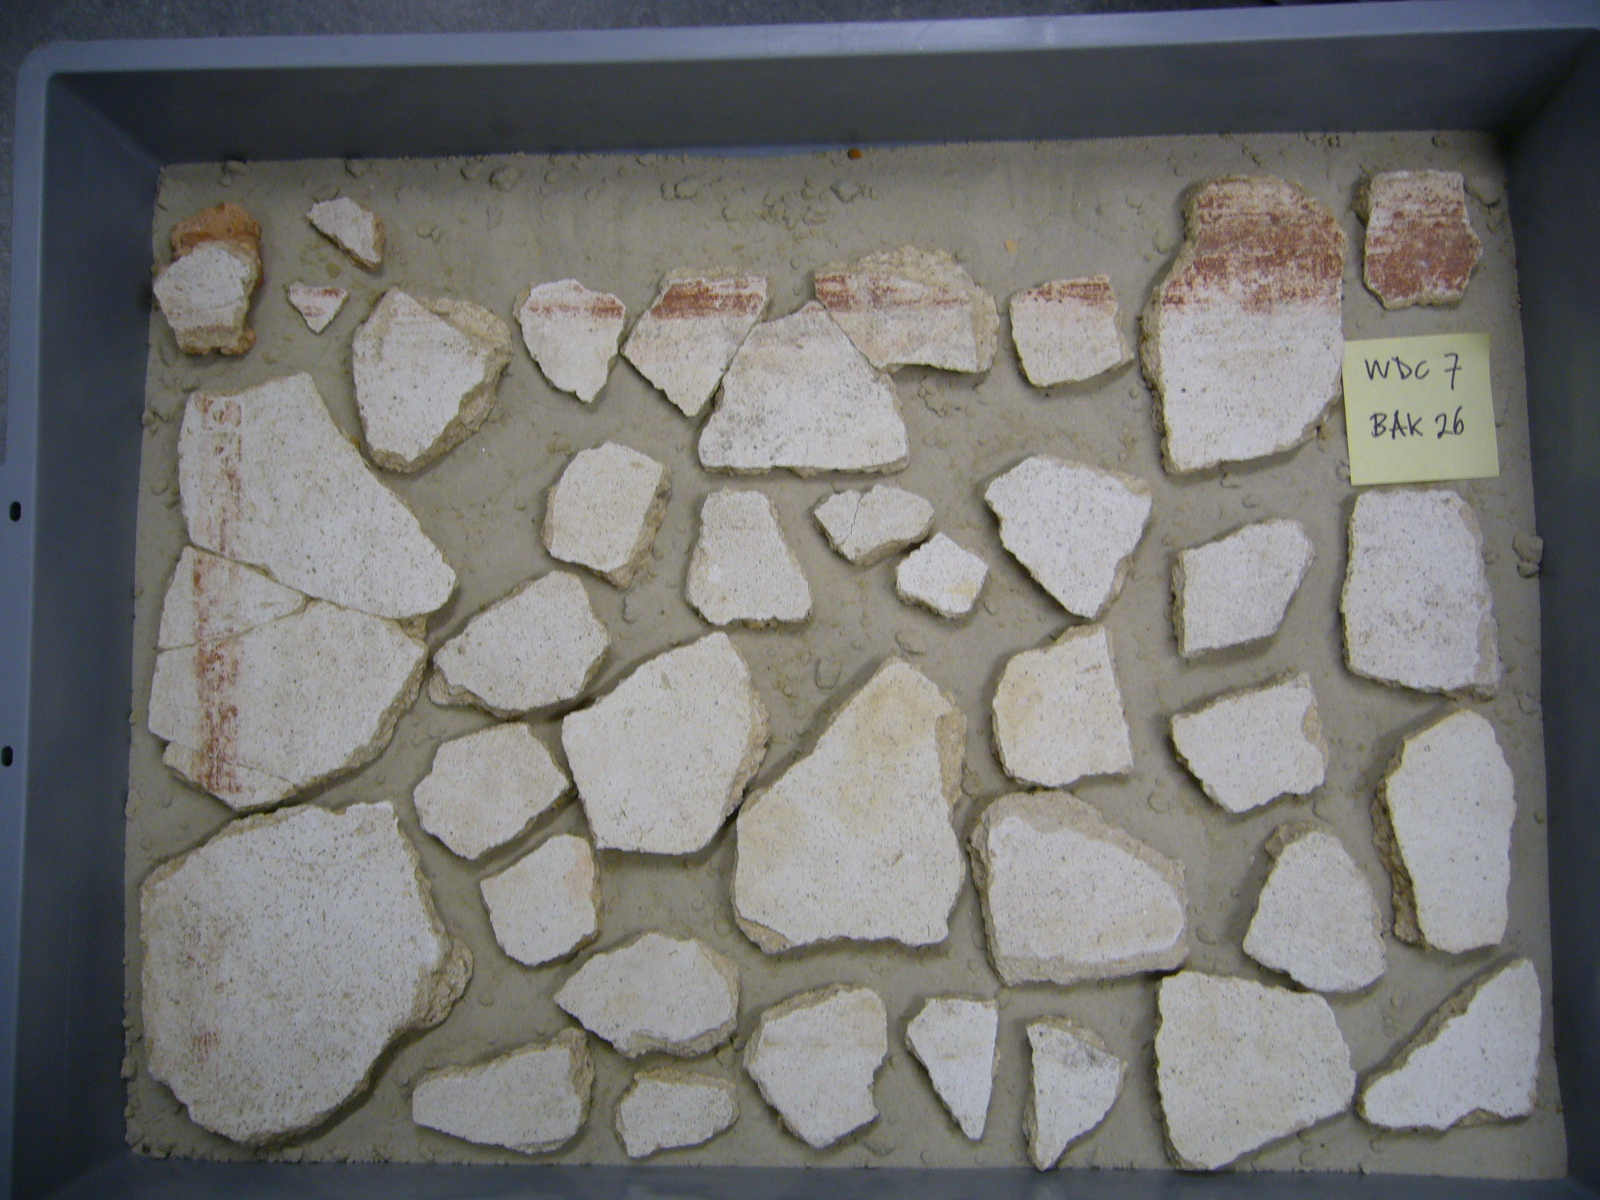
\includegraphics[width=0.6\columnwidth]{images/WDC7_26.JPG}
		\caption{Een bak vol fragmenten die rond dezelfde locatie zijn gevonden, sommige zijn reeds aan elkaar gezet.}
		\label{fig:bakinleiding}
	\end{center}
\end{figure}

De stukken met een nog zichtbaar geometrisch patroon of van de rand van het fresco zijn in vergelijking met de anderen eenvoudig met elkaar te verbinden. Zij zijn door een ervaren archeoloog zonder hulp in elkaar te passen. De overige fragmenten die minder duidelijke informatie bevatten wat betreft hun oorspronkelijke plaatsing of structuur zijn meer ingewikkeld om aan elkaar te puzzelen. Het menselijke visuele systeem is immers niet erg geschikt om grillige randen te vergelijken en aaneen te zetten. Het enige alternatief lijkt om lokaler te zoeken en elk fragment te vergelijken met elk ander fragment. Deze aanpak is praktisch onmogelijk, aangezien er miljoenen combinaties van fragmenten mogelijk zijn.\\

In deze context situeert zich het thera\footnote{Thera is de oude naam voor het huidige griekse eiland genaamd Santorini, waar het project voor het eerst in de praktijk werd toegepast.} project. Dit project probeert om het werk van de archeoloog te vergemakkelijken door middel van een software platform~\cite{Brown2008}. De
redenering achter het project is dat een computer deze ondankbare taak, voorgesteld in de vorige paragraaf, kan automatiseren. Dergelijk systeem werd in 2007 aan de \emph{Princeton} universiteit in Amerika geconcipieerd. Sindsdien is er tot op de dag van vandaag door verschillende onderzoekers van over de hele wereld aan gewerkt. De werking van het systeem wordt in het volgende hoofdstuk nader toegelicht.\\

Deze thesis draait rond het maken van een uitbreiding op het platform. De uitbreiding moet de gebruikers van het systeem in staat stellen om de beschikbare data op nieuwe manieren te gebruiken, te visualiseren, aan te passen en te delen met medeonderzoekers. Aangaande terminologie zullen een paar woorden veelvuldig terugkomen: de termen fragment, brokstuk of gewoonweg stuk verwijzen altijd naar een enkel gebroken deel van het originele fresco. De termen fragmentpaar, paar en voorstel zijn gereserveerd voor een aaneenkoppeling van twee fragmenten op een bepaalde plaats. Het valt te benadrukken dat twee fragmenten verschillende paren kunnen vormen indien zij elkaar op verschillende punten raken (ook al liggen die punten niet zo ver uit elkaar). Aangezien vele paren als mogelijke configuratie beschouwd kunnen worden, worden deze ook wel als voorstel aangeduid. Verder verwijst deze tekst meermaals naar (automatische) herkenners, dit zijn de identificatiealgoritmen die twee fragmenten aan elkaar proberen passen.\\

\section{Overzicht}
Hoofdstuk~\ref{hoofdstuk:overzicht} geeft een overzicht van het bestaande werk en hoofdstuk~\ref{hoofdstuk:doelen} geeft aan op welke vlakken het project zal uitgebreid worden en waarom. Vervolgens behandelt hoofdstuk~\ref{hoofdstuk:ontwerp} het algemene ontwerp van de applicatie. Hoofdstukken~\ref{hoofdstuk:database},~\ref{hoofdstuk:synchronisatie} en~\ref{hoofdstuk:modules} gaan dieper in op enkele specifieke implementaties van het project zoals de database, de synchronisatie en de modules. Tenslotte volgt een besluit in hoofdstuk~\ref{hoofdstuk:besluit}, en een verwijzing naar toekomstig werk in hoofdstuk~\ref{toekomst}.
